\section{Glove Block Design}

The glove block manages inputs from and outputs to the two gloves the player
wears while using the game. Two modules comprise the entire block.

\begin{figure}
\centering
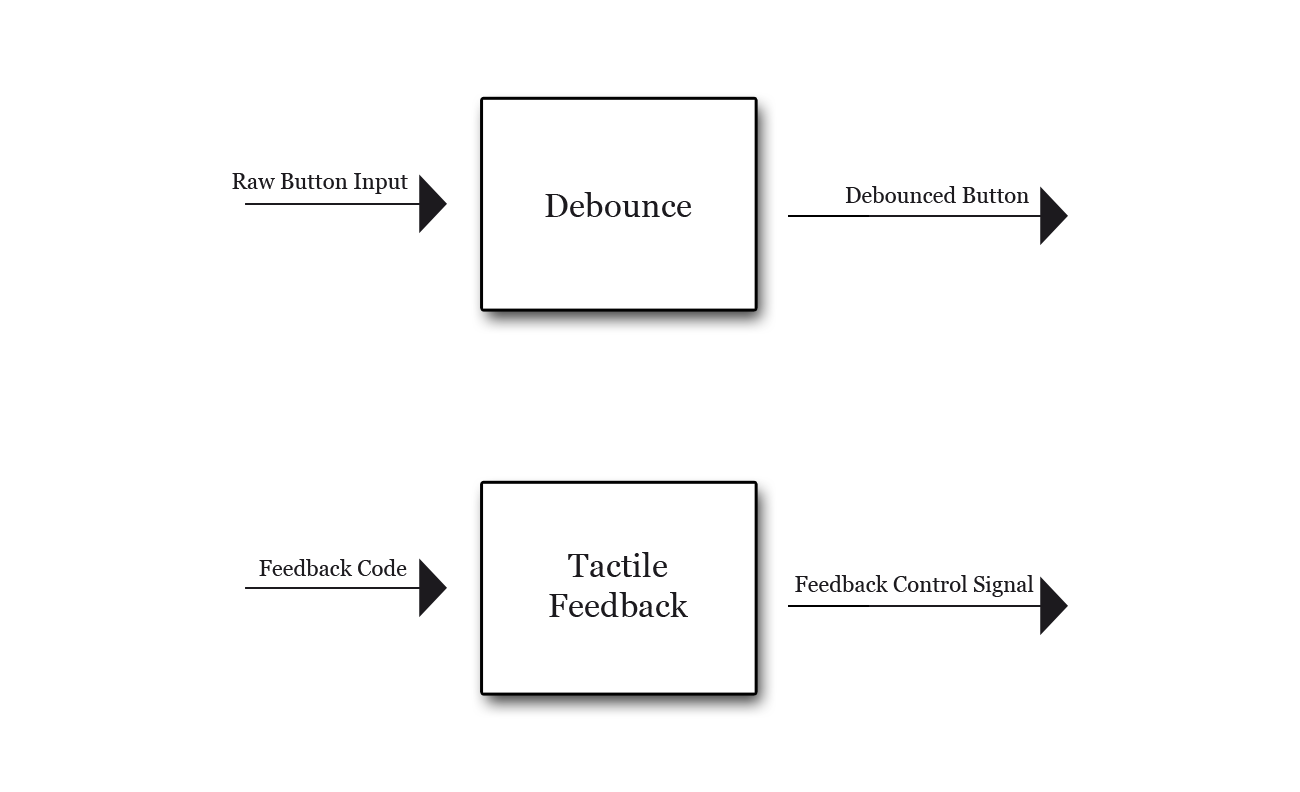
\includegraphics[scale=1]{img/glove.png}
\caption{The glove system is comprised of two data processing steps, one for the
debouncing of button input and the other for processing of tactile feedback duty
cycles.}
\label{fig:glove}
\end{figure}

\subsection{Tactile Feedback}

Tactile feedback is provided by this module, which processes an input from the
gameplay block and outputs a signal to power the motors attached to the user's
gloves. This game used only the most basic tactile feedback. If a hand was
touching a hold, the motors on that hand buzzed. As a result the module needed
only feed the signal through from the gameplay block to the relevant output on
the board. 

A modification of this game and potential place for future work is to add more
sophisticated feedback. The location of the buzzing on the player's palm could,
for example, indicate which direction they need to move in order to find a hold
and its strength could indicate how close they are to it.

\subsection{Debounce}

A simple debouncer syncronizes the noisy input from the flex sensors on the
player's gloves and debounces them, providing the clean signal as output to the
gameplay block.
